%! Author = itgramic
%! Date = 29.09.23

% Preamble

\section{Ausgangslage und Problemstellung}
\subsection{Das Kantonsspital Graubünden}
Das Kantonsspital Graubünden ist das Zentrumsspital der Südostschweiz, welches Teil der sogenannten Penta Plus Spitäler ist.
Die Penta plus Spitäler sind das Kantonsspital Baden, das Kantonsspital Winterthur, das Spitalzentrum Biel AG, das Kantonsspital Baselland, die Spital STS (Simmental-Thun-Saanenland) AG und eben das Kantonsspital Graubünden.

Das KSGR deckt dabei die Spitalregion Churer Rheintal ab
\begin{figure}[H]
    \centering
    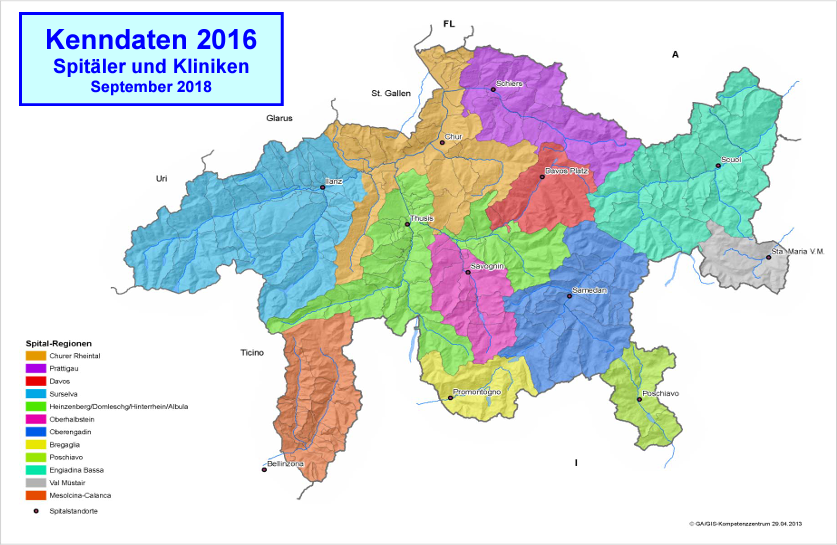
\includegraphics[width=1\linewidth]{source/introduction/initial_situation/gr_spitalregionen}
    \caption{Spitalregionen Kanton Graubünden\cite{ER2J77MB}}
    \label{fig:gr_spitalregionen}
\end{figure}

Seit dem 1. Januar 2023 betreibt das KSGR den Standort Walenstadt im Kanton St. Gallen und deckt primär den Wahlkreis Sarganserland ab.
\begin{figure}[H]
    \centering
    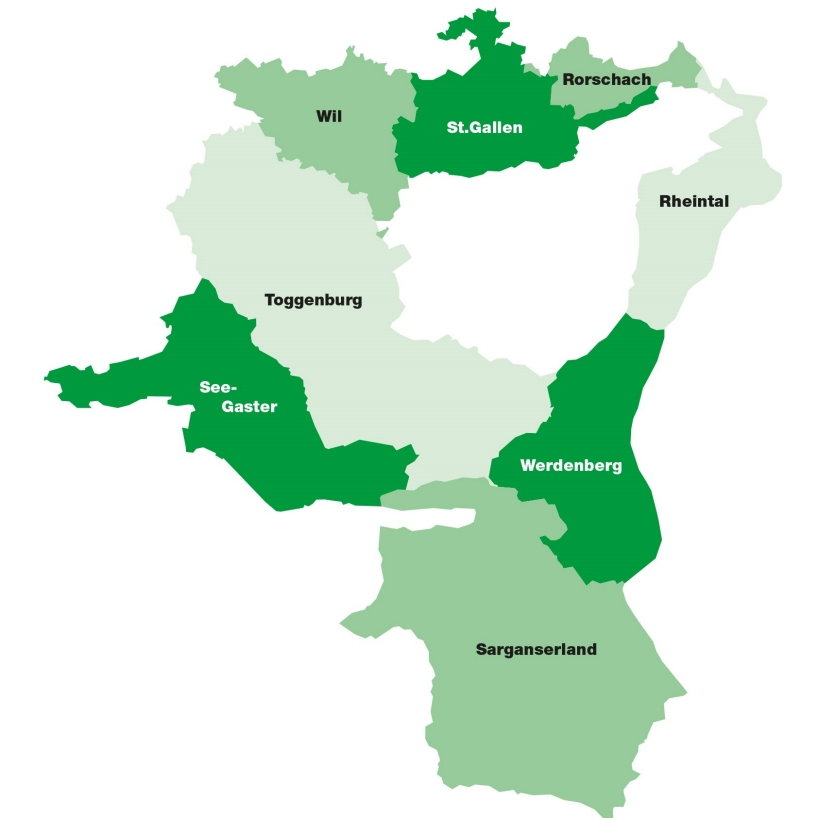
\includegraphics[width=0.75\linewidth]{source/introduction/initial_situation/sg_wahlkreise}
    \caption{Wahlkreise Kanton St. Gallen\cite{LEZ4SPDD}}
    \label{fig:sg_wahlkreise}
\end{figure}

Da dieser Wahlkreis der Spitalregion Rheintal Werdenberg Sarganserland zugeordnet ist, wird das KSGR auch im restlichen südlichen Teil der Spitalregion aktiv sein.
\begin{figure}[H]
    \centering
    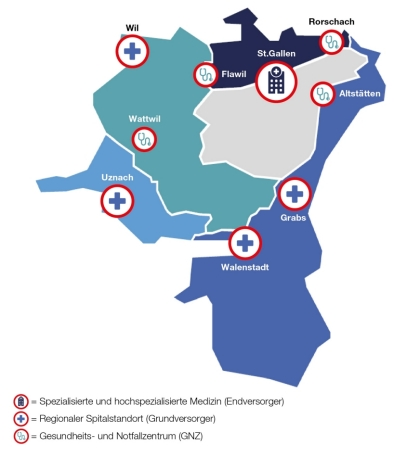
\includegraphics[width=0.5\linewidth]{source/introduction/initial_situation/sg_spitalregionen}
    \caption{Spitalregionen / Spitalstrategie Kanton St. Gallen\cite{3L8EIPUP}}
    \label{fig:sg_spitalregionen}
\end{figure}
\subsection{Die ICT des Kantonsspital Graubünden}
Das Kantonsspital Graubünden hat eine Matrixorganisation.
Die ICT ist ein eigenständiges Departement und gilt als sogenanntes Querschnittsdepartement, dh.
die ICT bedient alle anderen Departemente.
\begin{figure}[H]
    \centering
    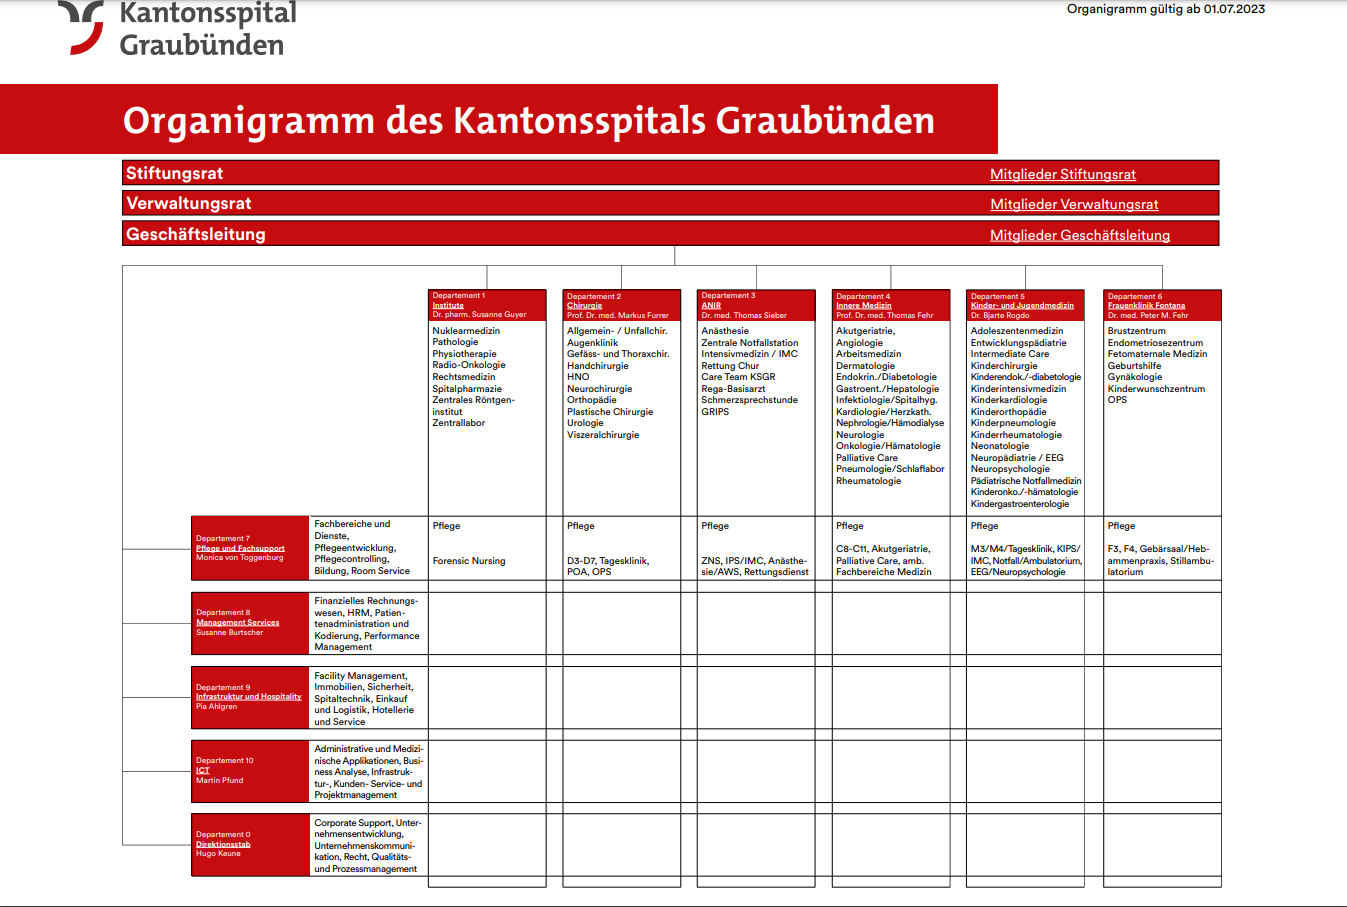
\includegraphics[width=1\linewidth]{source/introduction/initial_situation/Organigramm_KSGR}
    \caption{Organigramm Kantonsspital Graubünden}
    \label{fig:Organigramm_KSGR}
\end{figure}

Die ICT betreibt über 400 Applikationen die auf mehr als 1055 physische und virtuelle Server und Appliances.
Das Rückgrat der Infrastruktur ist dabei die Virtualisierungsplattformen VMware ESXi für Server und Citrix für die Thinclients der Enduser.
Es werden aber auch Dienstleistungen für andere Spitäler und Kliniken oder andere Einrichtungen des Gesundheitswesens erbracht.

Entsprechen wurde die ICT in ein Applikationsmanagement, ein Infrastrukturmanagement sowie einem unterstützenden Bereich aufgegliedert.
Das Applikationsmanagement wurde in je einen Bereich für die Administrativen und Medizinischen Applikationen aufgeteilt.
Das Infrastrukturmanagement wiederum wurde in den Bereich Netzwerk und Data Center, welcher für Server zuständig ist, aufgeteilt.
Der Bereich Business- und Prozessunterstützung beinhaltet je eine Abteilung für die Businessanalyse, das Projektmanagement und Benutzer- und Clientservices in der auch der Service-Desk untergebracht ist.
\begin{figure}[H]
    \centering
    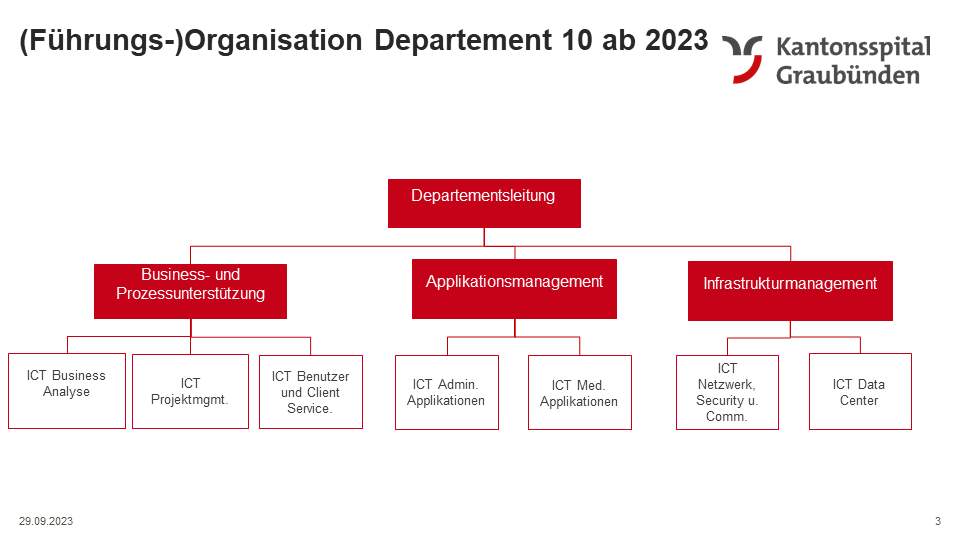
\includegraphics[width=1\linewidth]{source/introduction/initial_situation/Organigramm-D10}
    \caption{Organigramm Departement 10 - ICT}
    \label{fig:Organigramm_D10}
\end{figure}

Die Organisation der ICT wird sich aber bis spätestens zum Abschluss der Diplomarbeit noch verändern.
\subsection{Rolle in der ICT vom Kantonsspital Graubünden}
Meine Rolle im Kantonsspital Graubünden resp. in der ICT ist die eines DBA.
Diese Rolle ist in der Abteilung ICT Data Center.

Da die Kernsysteme auf Oracle Datenbanken und \Gls{HP-UX} laufen, bin ich primär \Gls{Oracle Database} DBA und manage das \Gls{HP-UX} in Zusammenarbeit mit HPE.
Die administrative Tätigkeit bei \Gls{HP-UX} besteht primär im Betrieb der \Gls{HP-UX} Cluster Packages (einer sehr
rudimentären Art von Containern), überwachen und erweitern des Filesystems, erweitern von \Gls{SAN} Storage Lunes für die Filesystem erweiterung, Erstellen von \Gls{PRTG}-Sensoren für
das Monitoring, SAP Printerqueue Management und andere Tasks die es noch auszuführen gibt.
Daneben bin ich auch für andere Datenbanken, teilweise aber nur begrenzt \Gls{Microsoft SQL Server}, \Gls{MySQL} /
\Gls{MariaDB} und vermehrt \Gls{PostgreSQL} zuständig.
Darüber hinaus bin ich Teilweise in die \Gls{Linux}-Administration involviert und betreue auch noch einige Windows Server für das Zentrale klinische Informationssystem.

\subsection{Ausgangslange}
Die meisten der über 400 Applikationen, die das KSGR betreibt, haben in den allermeisten Fällen ihre Daten in Datenbanksysteme speichern.
Entsprechend der Vielfalt der Applikationen existieren auch eine vielzahl an Datenbanksystemen und Versionen.

Basierend auf der Liste \textit{DB-Engines Ranking}\cite{TTVGIG2P} der Top-Datenbanksysteme .
Allerdings werden nicht alle Datenbanksysteme berücksichtigt, entweder weil das Datenbanksystem keine Client/Server Architektur hat oder nicht im Scope der IT oder des Projekts ist.

Folgende Datenbanken sind inventarisiert:
\begin{landscape}
\begin{table}[]
\resizebox{\columnwidth}{!}{%
\begin{tabular}{@{}llll@{}}
\toprule
\textbf{DBMS}                & \textbf{Datenbankmodell} & \textbf{Inventarisiert} & \textbf{Kommentar}                                                            \\ \midrule
\Gls{Oracle Database}                       & Relational, \Gls{NoSQL}, \Gls{OLAP}  & Ja                      &                                                                               \\
\Gls{MySQL}                        & Relational               & Ja                      &                                                                               \\
\Gls{Microsoft SQL Server}         & Relational, \Gls{NoSQL}, \Gls{OLAP}  & Nein                    & Werden separat administriert und sind daher nicht in diesem Inventar gelistet \\
\Gls{PostgreSQL}                   & Relational, \Gls{NoSQL}        & Ja                      &                                                                               \\
\Gls{MongoDB}                      & \Gls{NoSQL}                    & Ja                      &                                                                               \\
\Gls{Redis}                        & Key-value                & Ja                      &                                                                               \\
\Gls{Elasticsearch}                & Search engine            & Ja                      &                                                                               \\
\Gls{IBM DB2}                      & Relational               & Ja                      &                                                                               \\
\Gls{SQLite}                       & Relational               & Nein                    & Lokale Datenbank. Zudem wird die DB nicht via Netzwerk angesprochen           \\
\Gls{Microsoft Access}             & Relational               & Nein                    & Nicht im Scope der ICT                                                        \\
\Gls{Snowflake}                    & Relational               & Ja                      &                                                                               \\
\Gls{Cassandra}                    & Relational               & Ja                      &                                                                               \\
\Gls{MariaDB}                      & Relational               & Ja                      &                                                                               \\
\Gls{Splunk}                       & Search engine            & Ja                      &                                                                               \\
\Gls{Microsoft Azure SQL Database} & Relational, \Gls{NoSQL}, \Gls{OLAP}  & Nein                    & Datenbanken sind nicht On-Premise und somit nicht im Scope                    \\ \bottomrule
\end{tabular}%
}
\caption{Inventarisierte Datenbanksysteme}
\label{tab:Inventarisierte Datenbanksysteme}
\end{table}
\end{landscape}

Folgende Datenbanksysteme sind demnach im KSGR im Einsatz:
%\begin{longtable}{@{}lll@{}}
%\toprule
%\textbf{\Gls{RDBMS}}                   & \textbf{Summe RDBMS / Cluster / CDB / Instance} & \textbf{Summe Databases} \\* \midrule
%\endfirsthead
%%
%\endhead
%%
%\bottomrule
%\endfoot
%%
%\endlastfoot
%%
%\Gls{MariaDB}                 & 2                                      & 2               \\
%\Gls{MongoDB}                 & 2                                      & 2               \\
%\Gls{MySQL}                   & 28                                     & 50              \\
%\Gls{Oracle Database}         & 27                                     & 30              \\
%\Gls{PostgreSQL}              & 20                                     & 20              \\
%\Gls{Redis}                   & 1                                      & 1               \\* \midrule
%\textbf{Gesamtergebnis} & \textbf{80}                            & \textbf{105}    \\* \bottomrule
%\caption{Datenbankinventar}
%\label{Datenbankinventar}
%\end{longtable}
% neu mit latex generator
\begin{table}[H]


\begin{tabular}{llrrr}
\toprule
 & RDBMS & Instanz & Datenbanken & Appliance \\
\midrule
0 & MariaDB & 2 & 2 & 0 \\
1 & MongoDB & 2 & 2 & 0 \\
2 & MySQL & 28 & 50 & 3 \\
3 & Oracle Database & 27 & 30 & 0 \\
4 & PostgreSQL & 20 & 20 & 4 \\
5 & Redis & 1 & 1 & 0 \\
Gesamtergebnis &  & 80 & 105 & 7 \\
\bottomrule
\end{tabular}
\caption{Datenbankinventar} \label{db_inventory_per_rdbms}
\end{table}


Aufgeschlüsselt auf die Betriebssysteme auf denen die Datenbanken laufen, ergibt sich folgendes Bild:
%\begin{longtable}{@{}llrr@{}}
%\toprule
%\multicolumn{2}{l}{\textbf{OS / \Gls{RDBMS}}}     & \multicolumn{1}{l}{\textbf{Summe RDBMS / Cluster / CDB / Instance}} & \multicolumn{1}{l}{\textbf{Summe Databases}} \\* \midrule
%\endfirsthead
%%
%\endhead
%%
%\bottomrule
%\endfoot
%%
%\endlastfoot
%%
%\multicolumn{2}{l}{\textbf{\Gls{HP-UX}}}          & \textbf{21}                                                         & \textbf{24}                                  \\* \midrule
%             & \Gls{Oracle Database}s             & 21                                                                  & 24                                           \\
%\multicolumn{2}{l}{\textbf{\Gls{Linux}}}          & \textbf{26}                                                         & \textbf{48}                                  \\* \midrule
%             & \Gls{MariaDB}                      & 2                                                                   & 2                                            \\
%             & \Gls{MySQL}                        & 14                                                                  & 36                                           \\
%             & \Gls{Oracle Database}              & 1                                                                   & 1                                            \\
%             & \Gls{PostgreSQL}                   & 8                                                                   & 8                                            \\
%             & \Gls{Redis}                        & 1                                                                   & 1                                            \\
%\multicolumn{2}{l}{\textbf{Windows Server}} & \textbf{33}                                                         & \textbf{33}                                  \\* \midrule
%             & \Gls{MongoDB}                      & 2                                                                   & 2                                            \\
%             & \Gls{MySQL}                        & 14                                                                  & 14                                           \\
%             & \Gls{Oracle Database}s             & 5                                                                   & 5                                            \\
%             & \Gls{PostgreSQL}                   & 12                                                                  & 12                                           \\* \midrule
%\multicolumn{2}{l}{\textbf{Gesamtergebnis}} & \textbf{80}                                                         & \textbf{105}                                 \\* \bottomrule
%\caption{\mbox{Datenbankinventor - Nach Betriebssystemen aufgeschlüsselt}}
%\label{Datenbankinventar_per_OS}
%\end{longtable}
% neu mit latex generator
\begin{longtable}[H]{llrrr}

\toprule
 &  & Appliance & Datenbanken & Instanz \\
OS & RDBMS &  &  &  \\
\midrule
\endfirsthead
\caption[]{Datenbankinventor - Nach Betriebssystemen aufgeschlüsselt} \\
\toprule
 &  & Appliance & Datenbanken & Instanz \\
OS & RDBMS &  &  &  \\
\midrule
\endhead
\midrule
\multicolumn{5}{r}{Continued on next page} \\
\midrule
\endfoot
\bottomrule
\endlastfoot
HP-UX & Oracle Database & 0 & 24 & 21 \\
\cline{1-5}
\multirow[t]{5}{*}{Linux} & MariaDB & 0 & 2 & 2 \\
 & MySQL & 3 & 36 & 14 \\
 & Oracle Database & 0 & 1 & 1 \\
 & PostgreSQL & 4 & 8 & 8 \\
 & Redis & 0 & 1 & 1 \\
\cline{1-5}
\multirow[t]{4}{*}{Windows Server} & MongoDB & 0 & 2 & 2 \\
 & MySQL & 0 & 14 & 14 \\
 & Oracle Database & 0 & 5 & 5 \\
 & PostgreSQL & 0 & 12 & 12 \\
\cline{1-5}
Gesamtergebnis &  & 7 & 105 & 80 \\
\cline{1-5}
\caption{Datenbankinventor - Nach Betriebssystemen aufgeschlüsselt} \label{db_inventory_per_os}
\end{longtable}


Die Kernsysteme des Spitals werden auf Oracle Datenbanken (\Gls{Oracle Database})betrieben, die aktuell auf einer \Gls{HP-UX} betrieben werden.
Stand heute gibt es kein Clustersystem für die Open-Source Datenbanken wie \Gls{MariaDB}/\Gls{MySQL} oder \Gls{PostgreSQL}\@.

Durch die Einführung von \Gls{Kubernetes} als Containerplattform wird der Bedarf an \Gls{PostgreSQL} Datenbanken immer grösser.
Es werden in naher Zukunft auch verschiedene Oracle Datenbanken sowie \Gls{MySQL} Datenbanken auf \Gls{PostgreSQL} migriert werden.

Aktuell werden die Daten des \Gls{Zabbix} der Netzwerktechniker auf eine \Gls{MariaDB} Datenbank gespeichert, dies soll sich aber ändern.
Da das \Gls{Zabbix} alle Netzwerkgeräte Überwacht, pro Sekunde werden im Moment 1'200 Datenpunkte abgefragt und xxx in die Datenbank und wird im Laufe der Zeit mehrere Terrabyte gross werden.
\subsection{Problemstellung}
Zusammen mit den bestehenden \Gls{PostgreSQL}-Datenbankinstanzen werden die \Gls{PostgreSQL} Datenbanken in der Art, wie sie bisher Betrieben werden, nicht mehr Betreibbar sein.
Die bisherige Strategie erzeugt sehr viele Aufwände und provoziert Risiken, namentlich:
\begin{itemize}
    \item dezentrale Backups und fragmentierte Backup-Strategien
    \begin{itemize}
        \item Fehlende Kontrolle
        \item Wiederherstellbarkeit nicht garantiert
    \end{itemize}
    \item Verschiedene Betriebssysteme mit verschiedenen Versionen
    \begin{itemize}
        \item Fehlernder Überblick
        \item Veraltete Betriebssystem- und Datenbankversionen
        \item Grosser Administrationsaufwand
    \end{itemize}
    \item Uneinheitliche Absicherung und Härtung
    \begin{itemize}
        \item Hohe Angreifbarkeit
        \item Veraltete Betriebssystem- und Datenbankversionen
        \item Grosser Administrationsaufwand
    \end{itemize}
    \item Uneinheitliche HA-Fähigkeit
    \begin{itemize}
        \item Hohe Angreifbarkeit
        \item Veraltete Betriebssystem- und Datenbankversionen
        \item Grosser Administrationsaufwand
    \end{itemize}
\end{itemize}

Dadurch ergeben sich nach BSI folgende Risiken:
\begin{landscape}
\begin{table}[]
\resizebox{\columnwidth}{!}{%
\begin{tabular}{llllllllllll}
\hline
\multicolumn{4}{l}{}                                                                                                                                                                        &                                                                                                                                                                                                                                                                                                                                                                                                                                                                                                                                                                                                                                                                                                                                                                                                                              &                                                                                                                                                                                                                                                                                                                                                                                                                                                                                                                                                         & \multicolumn{2}{l}{}                                  & \multicolumn{4}{l}{Behandlung}                                                                                                                                                                                                                                 \\ \cline{9-12}
\multicolumn{4}{l}{\multirow{-2}{*}{Identifikation}}                                                                                                                                        & \multirow{-2}{*}{}                                                                                                                                                                                                                                                                                                                                                                                                                                                                                                                                                                                                                                                                                                                                                                                                           & \multirow{-2}{*}{}                                                                                                                                                                                                                                                                                                                                                                                                                                                                                                                                      & \multicolumn{2}{l}{\multirow{-2}{*}{Abschätzung}}     &                                                                                   & \multicolumn{2}{l}{Zielwert} &                                                                                                                                             \\ \cline{1-8} \cline{10-11}
ID & Schutzziel & \begin{tabular}[c]{@{}l@{}}Referenz\\ BSI 200-3\end{tabular} & Risiko                                                                                                     & Beschreibung / Ursache                                                                                                                                                                                                                                                                                                                                                                                                                                                                                                                                                                                                                                                                                                                                                                                                       & Auswirkung                                                                                                                                                                                                                                                                                                                                                                                                                                                                                                                                              & WS                        & SM                        & \multirow{-2}{*}{\begin{tabular}[c]{@{}l@{}}Massnahmen\\ ergreifen?\end{tabular}} & WS            & SM           & \multirow{-2}{*}{Massnahme}                                                                                                                 \\ \hline
1  & I          & G0.22                                                        & Manipulation von Informationen                                                                             & \begin{tabular}[c]{@{}l@{}}Durch veraltete Systeme die zudem unterschiedlich gut gehärtet und \\ gesichert sind (z.B. durch Verschlüsselung des Verkehrs oder der Daten auf dem Storage), \\ besteht das Risiko das Daten manipuliert werden\end{tabular}                                                                                                                                                                                                                                                                                                                                                                                                                                                                                                                                                                    & \begin{tabular}[c]{@{}l@{}}Die Auswirkungen reichen von einer Fehlfunktion des Systems \\ bis hin zum vollständigen Verlust der Integrität der Daten\end{tabular}                                                                                                                                                                                                                                                                                                                                                                                       & \cellcolor[HTML]{F8FF00}2 & \cellcolor[HTML]{F8FF00}4 & Ja                                                                                & 1             & 2            & \begin{tabular}[c]{@{}l@{}}Best-Practice bei Härtung der Systeme.\\ Redundanzen einführen\end{tabular}                                      \\
2  & A          & G0.25                                                        & Ausfall von Geräten oder Systemen                                                                          & \begin{tabular}[c]{@{}l@{}}Manche Datenbanken und deren Betriebssysteme sind sehr alt und sehr lange im Einsatz.\\ Einige dieser Systeme sind schon so alt, das keine Hotfixes,\\ Patches und Updates mehr erhältlich sind.\\ Hierdurch entsteht das Risiko, das Systeme Ausfallen\end{tabular}                                                                                                                                                                                                                                                                                                                                                                                                                                                                                                                              & \begin{tabular}[c]{@{}l@{}}Sofern keine HA-Architektur aufgebaut wurde,\\ ist die Verfügbarkeit ernsthaft gefährdet resp.\\ die Applikation steht nicht mehr zur Verfügung.\end{tabular}                                                                                                                                                                                                                                                                                                                                                                & \cellcolor[HTML]{F8FF00}4 & \cellcolor[HTML]{F8FF00}4 & Ja                                                                                & 2             & 2            & Redundanzen einführen                                                                                                                       \\
3  & C, I, A    & G0.26                                                        & Fehlfunktion von Geräten oder Systemen                                                                     & \begin{tabular}[c]{@{}l@{}}Manche Datenbanken und deren Betriebssysteme sind sehr alt und sehr lange im Einsatz.\\ Einige dieser Systeme sind schon so alt, das keine Hotfixes,\\ Patches und Updates mehr erhältlich sind.\\ Hierdurch entsteht das Risiko, das Systeme Fehlfunktionen erleiden.\\ \\ Allerdings versuchen Datenbanksysteme, die Auswirkungen so gering wie möglich zu halten.\end{tabular}                                                                                                                                                                                                                                                                                                                                                                                                                 & \begin{tabular}[c]{@{}l@{}}Fehlfunktionen können innerhalb von Datenbanksystemen\\ die Datenkonsistenz verletzen,\\ Daten können verloren gehen oder ungewollt von\\ Dritten und unberechtigten Personen eingesehen werden.\\ Systeme könnten nicht mehr oder nur noch eingeschränkt verfügbar werden.\\ \\ Daher sind sowohl Vertraulichkeit, Integrität und Verfügbarkeit gefährdet.\end{tabular}                                                                                                                                                     & 2                         & \cellcolor[HTML]{F8FF00}4 & Ja                                                                                & 2             & 2            & \begin{tabular}[c]{@{}l@{}}Systeme zentralisieren\\ Lifecycle etablieren\end{tabular}                                                       \\
4  & C, I, A    & G0.27-1                                                      & Ressourcenmangel (personelle Ressourcen)                                                                   & \begin{tabular}[c]{@{}l@{}}Aufgrund der sehr heterogenen Landschaft ist der\\ Administrationsaufwand für die jetzigen Systeme sehr gross.\\ Zu gross, als das für jede Datenbank und deren Betriebssystem\\ die notwendige Zeit für eine bedarfsgerechte Administration erbracht werden kann.\\ \\ Dadurch bleiben Fehler länger unentdeckt, Hotfixes, Patches, Updates und Upgrades\\ können nicht oder nicht zur richtigen Zeit eingespielt werden.\\ \\ Bei einem akuten Problemfall ist nicht garantiert,\\ das die Leute erreichbar sind, die notwendig sind\end{tabular}                                                                                                                                                                                                                                               & \begin{tabular}[c]{@{}l@{}}Die Auswirkungen können vielfältig sein,\\ abhängig davon welcher Aspekt unter dem Ressourcenmangel leidet.\\ \\ Grundsätzlich wird aber sowohl die Vertraulichkeit,\\ Integrität und Verfügbarkeit gefährdet.\end{tabular}                                                                                                                                                                                                                                                                                                  & \cellcolor[HTML]{F8FF00}3 & 3                         & Ja                                                                                & 2             & 3            & Systeme zentralisieren                                                                                                                      \\
5  & A          & G0.27-2                                                      & Ressourcenmangel (technische Ressourcen)                                                                   & \begin{tabular}[c]{@{}l@{}}Kann auftreten wenn Ressorucenwachstum zu spät bemerkt wird.\\ So kann die CPU Usage oder das Memory Usage schnell anwachsen.\\ Auch der Storage eines Betriebssystems kann nicht mehr ausreichend für ein System werden.\end{tabular}                                                                                                                                                                                                                                                                                                                                                                                                                                                                                                                                                            & \begin{tabular}[c]{@{}l@{}}Wenn die CPU- und Memory-Usage über einen gewissen Schwellwert geht,\\ fängt das Betriebssystem an zu Priorisieren.\\ Dies wird primär der Endanwender in form von Performance Einbussen bemerken.\\ Im schlimmsten Fall steht eine Anwendung nicht mehr zur Verfügung.\\ \\ Gefährlicher sind Storage Overflows, besonders wenn die Datenbank\\ nicht mehr alle Informationen schreiben konnte,\\ die sie für einen korrekten Neustart benötigte.\\ \\ Doch die folgen bleiben nichtsdesto trotz überschaubar.\end{tabular} & \cellcolor[HTML]{F8FF00}2 & 2                         & Ja                                                                                & 1             & 2            & Monitoring verschärfen                                                                                                                      \\
6  & C, I, A    & G0.31                                                        & \begin{tabular}[c]{@{}l@{}}Fehlerhafte Nutzung oder Administration\\ von Geräten und Systemen\end{tabular} & \begin{tabular}[c]{@{}l@{}}Durch die Vielfalt an Datenbankversionen und Betriebssystemen und\\ Plattformen worauf diese betrieben werden,\\ besteht allen voran das Risiko einer Fehlerhafter Administration und Konfiguration.\end{tabular}                                                                                                                                                                                                                                                                                                                                                                                                                                                                                                                                                                                 & \begin{tabular}[c]{@{}l@{}}Abhängig davon, welche Fehler gemacht wurden können\\ die Auswirkungen auch stark variieren.\\ Sie reichen von fehlender Verschlüsselung bis hin zu nicht vorhandenem\\ Backup mit nicht mehr gesicherter Wiederherstellbarkeit von Systemen.\\ \\ Daraus erschliesst sich das auch bei diesem Risiko die Vertraulichkeit,\\ Integrität und Verfügbarkeit gefährdet ist.\end{tabular}                                                                                                                                        & \cellcolor[HTML]{F8FF00}4 & 3                         & Ja                                                                                & 2             & 3            & Systeme zentralisieren                                                                                                                      \\
7  & C, I, A    & G0.32                                                        & Missbrauch von Berechtigungen                                                                              & \begin{tabular}[c]{@{}l@{}}Obwohl das Microsoft Active Directory die Zentrale Benutzerverwaltung ist,\\ sind die wenigsten Datenbanken an dieses angeschlossen.\\ Hinzu kommt der umstand, das in der Vergangenheit jeder Softwarelieferant\\ sein eigenes Benutzerkonzept mitgebracht hat,\\ auch bei den Datenbankzugängen.\\ \\ Multipliziert mit der Anzahl der unterschiedlichsten Datenbanken,\\ Betriebssystemen und Applikationen entsteht das Risiko,\\ das Berechtigungen Wissendlich oder Unwissendlich missbraucht werden.\end{tabular}                                                                                                                                                                                                                                                                          & \begin{tabular}[c]{@{}l@{}}Der Wissentliche oder Unwissentliche Missbrauch von Berechtigungen\\ kann verheerende Auswirkungen haben.\\ Unter anderem können Daten missbräuchlich abgezogen werden,\\ Daten manipuliert oder das ganze System komplett zerstört werden.\end{tabular}                                                                                                                                                                                                                                                                     & 2                         & \cellcolor[HTML]{F8FF00}4 & Ja                                                                                & 2             & 2            & \begin{tabular}[c]{@{}l@{}}Systeme zentralisieren\\ \\ Übergreifendes Berechtigungskonzept einführen\\ Monitoring der Zugriffe\end{tabular} \\
8  & A, I       & G0.45                                                        & Datenverlust                                                                                               & \begin{tabular}[c]{@{}l@{}}Verschiedene Datenbanken sind Standalone Cluster (Instanzen)\\ welche über keinen Failover-Mechanismus verfügen.\\ \\ Zudem wurden die meisten Datenbanken nur mittels Snapshots oder einem\\ Filesystem Backup gesichert, nicht über eine eigentliche Sicherung mittels WAL.\\ Gerade die fehlende WAL-Archivierung führt im Backupfall dazu,\\ das alle Transaktionen die zwischen dem letzten Backup nicht mehr vorhanden sind.\\ \\ Hinzu kommt, das für die meisten Datenbanken hohe Sicherungsintervalle\\ von einmal pro Stunde oder gar nur einmal  am Tag gewählt wurde.\\ \\ Ein weiterer Aspekt des Risikos besteht in der tatsache,\\ das aufgrund der grossen Anzahl Datenbanken und deren\\ Heterogenität nur wenige Backups auch wirklich regelmässig geprüft werden.\end{tabular} & \begin{tabular}[c]{@{}l@{}}Aus dem Risiko ergeben sich zwei Auswirkungen,\\ die aber beide ein hohes Mass an Schaden verursachen können.\\ \\ Erstens könnten Backups gar nicht mehr Wiederhergestellt werden,\\ dies hätte dann einen Totalen Datenverlust zur Folge.\\ Die zweite Ursache erwächst auf der fehlenden WAL-Archivierung,\\ dadurch können zwar die Daten bis zu einem Zeitpunkt X Wiederhergestellt\\ werden allerdings sind diese dann nicht zwingend Konsistent.\end{tabular}                                                         & \cellcolor[HTML]{F8FF00}4 & \cellcolor[HTML]{F8FF00}5 & Ja                                                                                & 1             & 3            & \begin{tabular}[c]{@{}l@{}}Systeme zentralisieren\\ Einheitliches Backupkonzept\\ Regelmässige Restore-Tests\end{tabular}                   \\ \cline{5-12}
\end{tabular}%
}
\caption{Risiko-Matrix aktuelle Situation PostgreSQL Datenbanken}
\label{tab:riskmatrix-postgresql}
\end{table}
\end{landscape}

\begin{figure}[H]
    \centering
    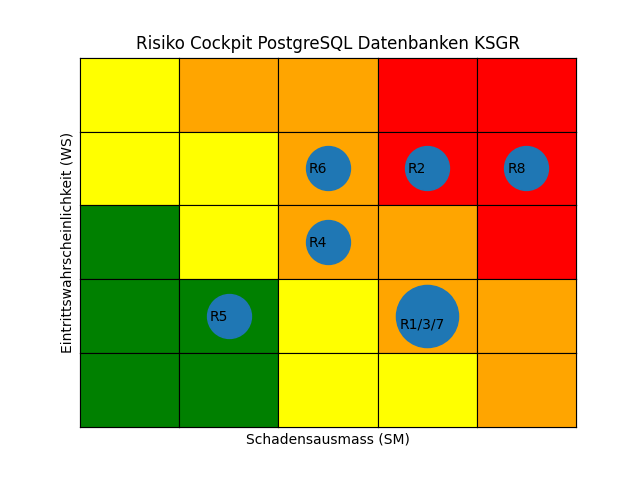
\includegraphics[width=1\linewidth]{source/riskmatrix/riskmatrixproblem}
    \caption{Risiken bestehende Lösung}
    \label{fig:riskmatrixproblem}
\end{figure}

% Python matplot risk management => versuchen
%https://stackoverflow.com/questions/62154079/risk-matrix-with-pythyon

Daraus ergeben sich folgende Strategien und Handlungsfelder um die Massnahmen zur Risikominimierung umzusetzen:
\begin{itemize}
    \item Systemabsicherung erarbeiten und einsetzen
    \item HA-Clustering einführen um die Redundanz zu gewährleisten und Systeme zentral verwalten und betreiben zu können
    \item Lifecycle-management für Datenbanken und Betriebssysteme erarbeiten und einsetzen
    \item Backupkonzept erarbeiten
    \item Berechtigungskonzept erarbeiten und einführen
\end{itemize}

Mit diesen Massnahmen lassen sich die Risiken gesenkt werden:
\begin{figure}[H]
    \centering
    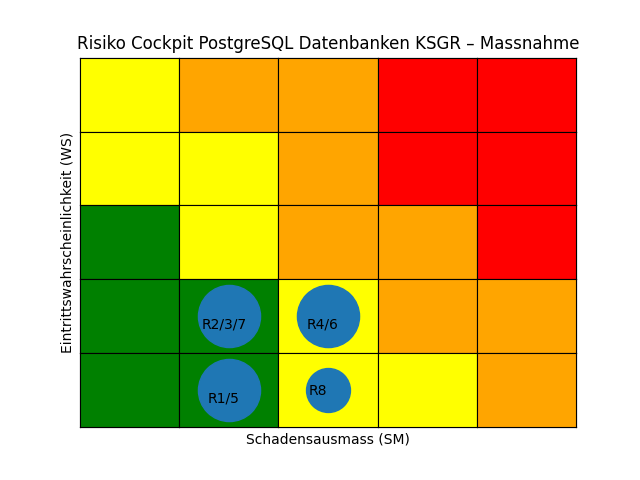
\includegraphics[width=1\linewidth]{source/riskmatrix/Riskmatrixproblem-massnahmen}
    \caption{Risiken bestehende Lösung mit Massnahmen}
    \label{fig:riskmatrixproblem-massnahmen}
\end{figure}